%----------------------------------------------------------------------------------------
%	PACKAGES AND OTHER DOCUMENT CONFIGURATIONS
%----------------------------------------------------------------------------------------

\documentclass[12pt]{article}

\usepackage{polski}
\usepackage[polish]{babel}
\usepackage[utf8]{inputenc}
\usepackage{datetime}
\usepackage{graphicx}
\usepackage{tikz}
\usepackage{amsmath}
\usepackage{epstopdf}
\usepackage{multirow}
\usepackage{tabularx}
%\usepackage[colorlinks=true]{hyperref}
%\usepackage[all]{hypcap}
%\usepackage{showframe} 
\usepackage{geometry}
 \geometry{
 	a4paper, 
 	left	=20mm,
 	right	=20mm,
 	top		=20mm,
 	bottom	=20mm,
 }
 
%----------------------------------------------------------------------------------------
 
%----------------------------------------------------------------------------------------
% DATES
%----------------------------------------------------------------------------------------

\renewcommand{\dateseparator}{.}
\newdate{exercise_date}{01}{06}{2015}

%----------------------------------------------------------------------------------------

%----------------------------------------------------------------------------------------
% TIKZ PACKAGES
%----------------------------------------------------------------------------------------

\usetikzlibrary{arrows}

%----------------------------------------------------------------------------------------

\begin{document}
 
\begin{titlepage}

\newcommand{\HRule}{\rule{\linewidth}{0.5mm}}
% Defines a new command for the horizontal lines, change thickness here

\center
% Center everything on the page
 
%----------------------------------------------------------------------------------------
%	LOGO SECTION
%----------------------------------------------------------------------------------------


\includegraphics[width=6cm]{../res/img/logo.png}\\[1cm]
% Include a department/university logo - this will require the graphicx package
 
%----------------------------------------------------------------------------------------
 
%----------------------------------------------------------------------------------------
%	HEADING SECTIONS
%----------------------------------------------------------------------------------------

\textsc{\LARGE Akademia Górniczo-Hutnicza \\[0.2cm]
im. Stanisława Staszica w Krakowie}\\[1.5cm]
% Name of your university/college

\textsc{\Large Podstawy Automatyki}\\[0.5cm]
% Major heading such as course name

%----------------------------------------------------------------------------------------
%	TITLE SECTION
%----------------------------------------------------------------------------------------

\HRule \\[0.5cm]
{ \huge \bfseries Dyskretne układy regulacji \\[0.3cm] oraz \\[0.5cm] Analiza
serwomechanizmu \\[0.2cm] przekaźnikowego z wykorzystaniem płaszczyzny
fazowej}\\[0.3cm]
% Title of your document
\HRule \\[1.5cm]
 
%----------------------------------------------------------------------------------------
%	AUTHOR SECTION
%----------------------------------------------------------------------------------------

% \begin{minipage}{0.4\textwidth}
% \begin{flushleft} \large
% \emph{Author:}\\
% Konrad \textsc{Adasiewcz} % Your name
% \end{flushleft}
% \end{minipage}
% ~
% \begin{minipage}{0.4\textwidth}
% \begin{flushright} \large
% \emph{Supervisor:} \\
% dr inż. Paweł \textsc{Rotter} % Supervisor's Name
% \end{flushright}
% \end{minipage}\\[4cm]

% If you don't want a supervisor, uncomment the two lines below and remove the section above
\flushright
\Large \emph{Autorzy:}\\
Konrad \textsc{Adasiewcz}\\[0.1cm] % Your name
Michał \textsc{Maciejewski}\\[3cm] % Your name

%----------------------------------------------------------------------------------------
%	DATE SECTION
%----------------------------------------------------------------------------------------
Data wykonania ćwiczenia: \\
{\large \displaydate{exercise_date}}\\[1cm]


\vfill % Fill the rest of the page with whitespace

\end{titlepage} 

\section{Wstęp}

Projektowanie sterowników systemów automatyki jest zadaniem złożonym,
wymaga od projektanta znajomości poza aspektami samej implementacji sterownika
znajomości platformy sprzętowej na której owy sterownik będzie uruchamiany.
Istnieją jednak zestawy narzędzi, które pozwalają zmniejszyć do minimum
wymagania dotyczące znajomości platformy sprzętowej sterownika, poprzez
separację projektanta od warstwy sprzętowej a nawet od warstwy programowej na
poziomie języka programowania. Jednym z takich zestawów jest Matlab-Simulink z
biblioteką RTI dla karty dSpace S1005 oraz Controldesk. Taki zestaw został użyty
podczas laboratorium.

\section{Cel ćwiczenia}

Celem ćwiczenia jest zaprojektowanie sterownika w pakiecie Matlab-Simulink,
uruchamianego na karcie dSpace S1005, pozwalającego kontrolować 3 główne osie
robota IRp-6 oraz interfejsu graficznego użytkownika w programie ControlDesk.
Projektowany sterownik powinien udostępniać następujące funkcjonalności:

\begin{itemize}
  \item Sterowanie napędów: serwomechanizmy dla poszczególnych osi z
  uwzględnieniem ograniczeń dla wartości zadanych kątów
  \item Bazowanie robota
  \item Pozycjonowanie w układzie współrzędnych konfiguracyjnych w trybach:
  ręcznym oraz wyzwalanym
  \item Zadawanie prędkości roboczej ruchu
  \item Koordynacja prędkości ruchu
  \item Implementacja problemu kinematyki prostej dla sterowanego robota
\end{itemize}

\newpage

\section{Implementacja sterownika}

\subsection{Sterowanie napędów: serwomechanizmy dla poszczególnych osi z
uwzględnieniem ograniczeń dla wartości zadanych kątów}

\begin{figure}[!htb]
    \begin{center}
        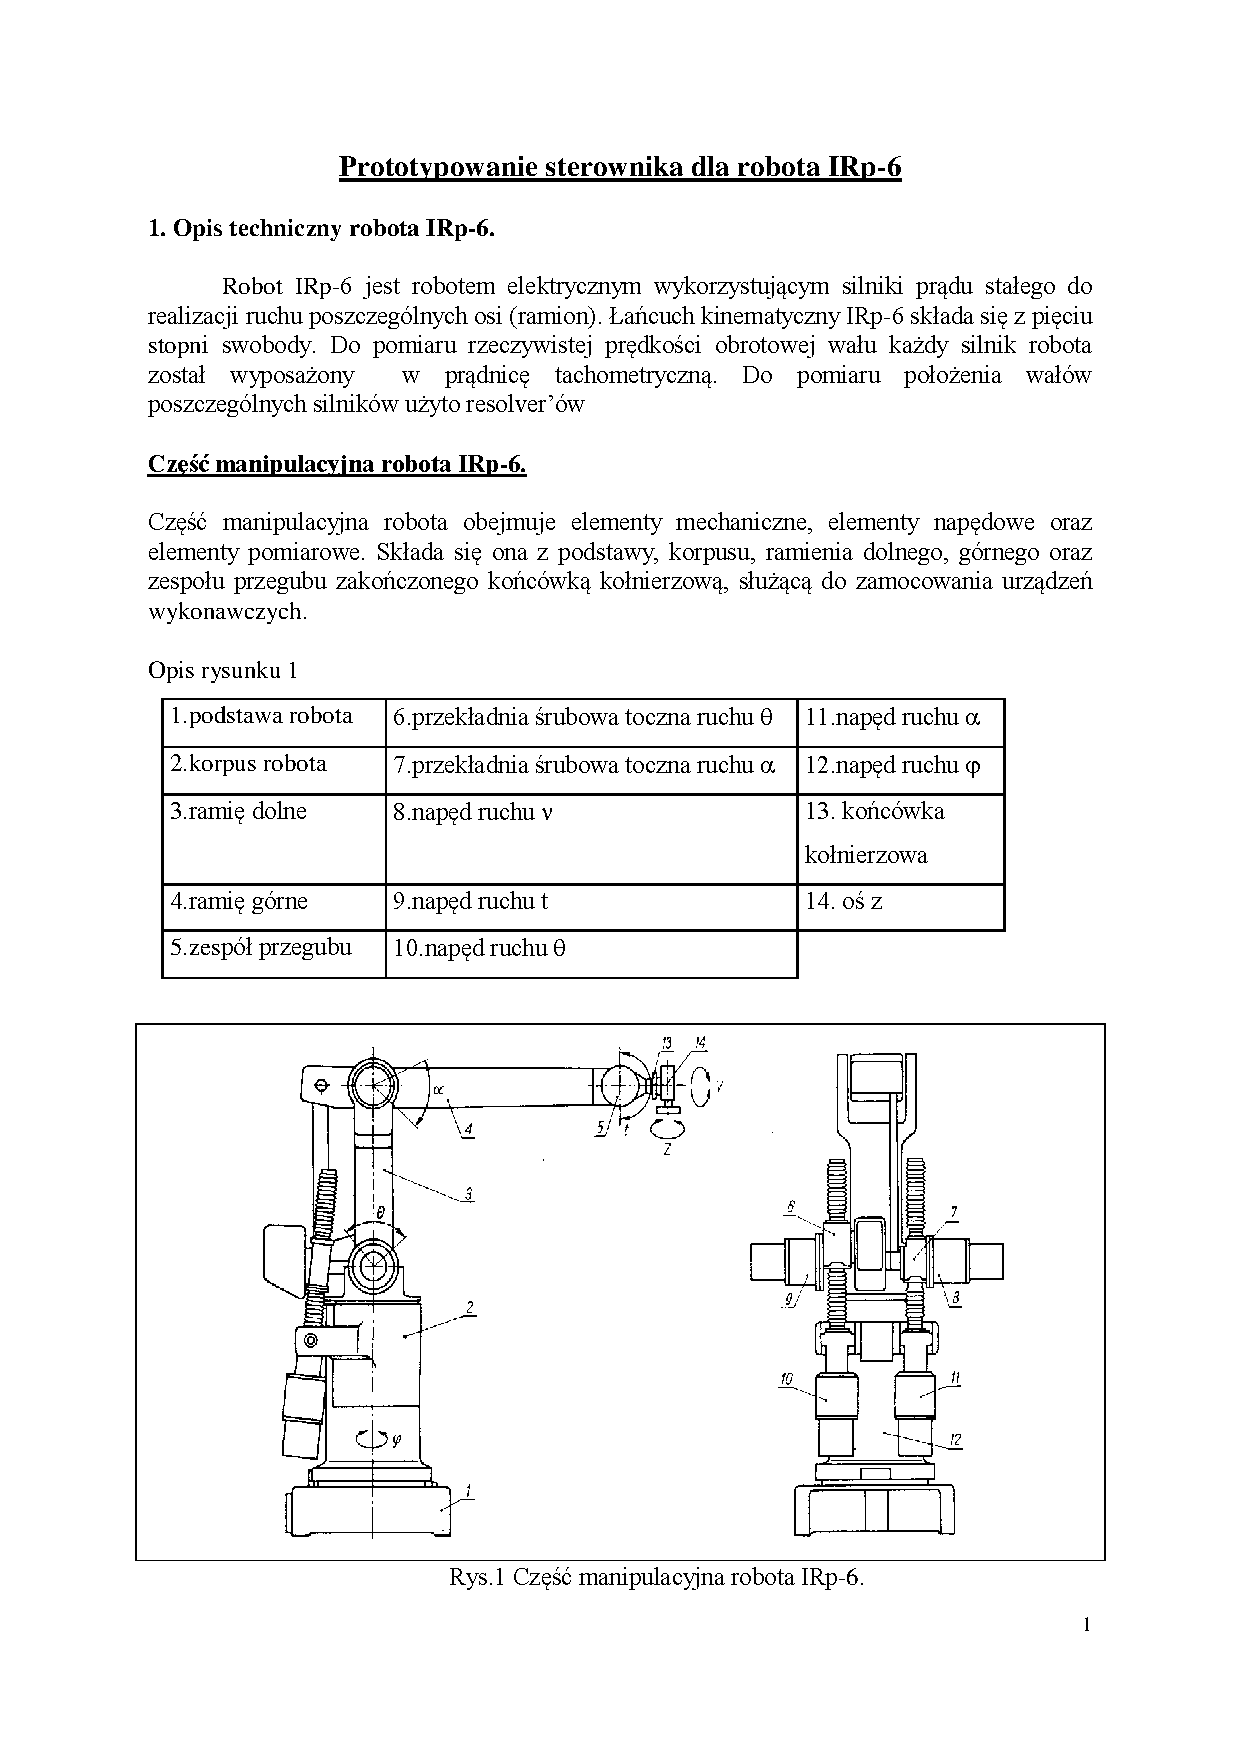
\includegraphics[page=1,width=17cm,trim=2.5cm 3.5cm 3cm 17.5cm,clip]
        {../res/img/ster_irp.pdf}
    \end{center}
    \caption{Część manipulacyjna robota}\label{rys:manip}
\end{figure}

W dalszej części sprawozdania zostały przyjęte następujące oznaczenia kątów,
odpowiadające kątom oznaczonym na rysunku \ref{rys:manip}:
\begin{center} 
    \begin{tabular}{lll}
        $\phi_1$ & $=$ & $\varphi$\\[0.1cm]
        $\phi_2$ & $=$ & $\theta$\\[0.1cm]
        $\phi_3$ & $=$ & $\alpha$
    \end{tabular}\\[0.1cm]
\end{center}

Do sterowania poszczególnymi osiam robota został wykorzystany regulator
proporcjonalny ze stałym wzmocnieniem $K_p = 0.5$. Również nieużywane osie
zostały zamknięte w pętlę sprzężenia zwrotnego z identycznym sterownikiem jak
dla kontrolowanych osi, jednak ze stałą wartością zadaną równą 0. Dodatkowo
zostały uwzględnione ograniczenia wartości zadanej kątów osi. Zadane
ograniczenia to:
\begin{center}
    \begin{tabular}{lll}
        $\phi_1$ & $\in$ & $[-160,160]$\\[0.1cm]
        $\phi_2$ & $\in$ & $[-40,40]$\\[0.1cm]
        $\phi_3$ & $\in$ & $[-25,40]$
    \end{tabular}\\[0.1cm]
    $|\phi_2-\phi_3|<40$
\end{center}

\newpage

\subsection{Bazowanie robota}

Bazowanie sterowanych osi robota polega na sterowaniu silnikami w otwartej pętli
sprzężenia zwrotnego, ze stałym sterowaniem, aż do momentu ustawienia się
ramienia robota w pozycji bazowej. O znajdowaniu się osi w pozycji bazowej
stanowi odczyt z odpowiednych czujników typu logicznego(w pozycji bazowej, lub
nie w pozycji bazowej). Na ich podstawie bazowanie zostaje zakończone, pętla
sprzężenia zwrotnego zamknięta, a wartość zadana kąta wyzerowana. Jednak aby
taka konfiguracja mogła działać, osie robota przed rozpoczęciem operacji
bazowania muszą być ustawione tak, aby podawane sterowanie zbliżało je do
pozycji bazowej, w przeciwnym wypadku bazowanie nie przebiegnie poprawnie.

\subsection{Pozycjonowanie w układzie współrzędnych konfiguracyjnych w trybach: ręcznym oraz
wyzwalanym}

Do zadawania pozycji robota zostały zaimplementowane dwa tryby pracy:

\begin{itemize}
  \item tryb pracy ręcznej
  \item tryb pracy wyzwalanej
\end{itemize}

W trybie pracy ręcznej ramiona robota natychmiast reagują na zmiany zadanych
wartości kątów, natomiast tryb pracy wyzwalanej wymaga jeszcze dodatkowego
pozwolenia na ruch robota po zadaniu kątów ramion(tutaj będzie to wciśnięcie
przycisku w Controldesku).

\subsection{Zadawanie prędkości roboczej ruchu}

Zadawanie prędkości silników zostało zrealizowane jako iloczyn wartości
sterowania regulatora i współczynnika z zakresu $S \in \{0.01,1\}$. Wartość
współczynnika prędkości nie może być zerowa, ponieważ jest to jednoznaczne z
otwarciem pętli sprzężenia zwrotnego i co za tym idzie utraty kontroli nad
położeniem silników.

\subsection{Koordynacja prędkości ruchu}

Zadaniem koordynacji prędkości ruchu silników jest takie sterowanie ramionami
robota aby w trybie wyzwalanym wszystkie ruchy zakończyły się w tym samym
momencie. Efekt taki można uzyskać kontrolując prędkości silników na podstawie
uchybów poszczególnych osi robota. Wartości współczynników prędkości
poszczególnych osi dane są zależnością:

\begin{equation*}
    c_i = \dfrac{|\varepsilon_i|}{\displaystyle\max_{j=1,2,3}(|\varepsilon_j|)}
    ,\hspace{0.5cm}i=1,2,3
\end{equation*}

\subsection{Implementacja problemu kinematyki prostej dla sterowanego robota}

Zadanie problemu kinematyki prostej polega na obliczeniu pozycji końcówki
manipulatora robota we współrzędnych kartezjańskich na podstawie współrzędnych
konfiguracyjnych. Współrzędne końcówki robota zostały obliczone na podstawie
zależności:

\begin{center}
    \begin{tabular}{lll}
        $x$ & $=$ & $\cos\phi_1\left[p_3\cos(-\phi_3) +
                                     p_2\cos(90 - \phi_2)\right]$ \\[0.2cm]
        $y$ & $=$ & $\sin\phi_1\left[p_3\cos(-\phi_3) +
                                     p_2\cos(90 - \phi_2)\right]$ \\[0.2cm]
        $z$ & $=$ & $p_3\sin(-\phi_3) + p_2\sin(90 - \phi_2) + p_1$
    \end{tabular}
\end{center}

gdzie $p_1=700[mm]$, $p_2=450[mm]$, $p_3=670[mm]$

\newpage

\section{Panel operatorski}

W celu przetestowania działania sterownika wymagana jest budowa panelu
operatorskiego umożliwiającego komunikację ze sterownikiem robota uruchomionym
na karcie dSpace. Został przez nas zaprojektowany prosty panel umożliwiający
sterowanie i odczyt wszystkich przewidzianych w ćwiczeniu opcji sterownika.

\begin{figure}[!htb]
    \begin{center}
        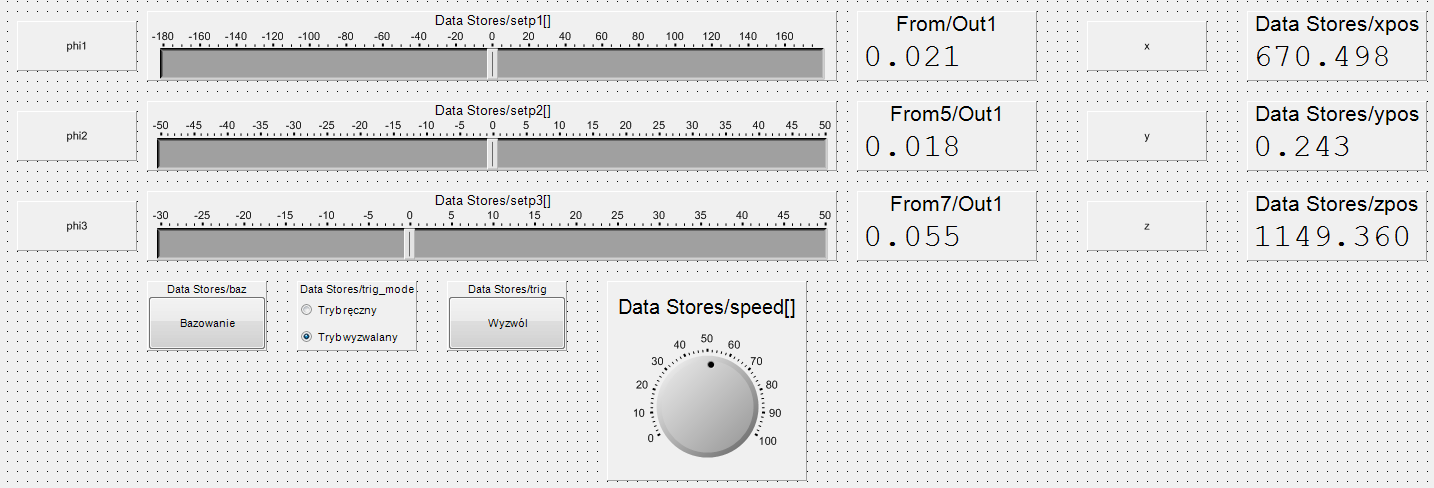
\includegraphics[width=17cm]
        {../res/img/panel.png}
    \end{center}
    \caption{Panel operatorski}
\end{figure}

Do elementów panelu należą:

\begin{itemize}
  \item Suwaki umożliwiające zadanie kątów trzech ramion robota zarówno dla
  pracy ręcznej jak i wyzwalanej
  \item Przycisk uruchamiający procedurę bazowania
  \item Radio button przełączający między trybami pracy ręcznej i wyzwalanej
  \item Przycisk zezwalający na ruch w trybie pracy wyzwalanej
  \item Pokrętło umożliwiające zadanie prędkości pracy silników
  \item Kontrolki odczytujące aktualne pozycje kątowe ramion robota
  \item Kontrolki odczytujące aktualną pozycję kartezjańską końcówki robota 
\end{itemize}

\section{Wnioski}

Korzystanie z pakietów i sprzętu typu Matlab-Simulink z biblioteką RTI dla karty
dSpace S1005 oraz Controldesk, znacznie przyspiesza proces implementacji
sterownika poprzez zwolnienie projektanta z wielu aspektów nieistotnych z punktu
widzenia budowanej aplikacji sterownika jak np. budowa i obsługa platformy
sprzętowej. Użycie uniwersalnej warstwy projektowania sterownika jaką jest
Matlab-Simulink dodatkowo umożliwia proste jego przenoszenie pomiędzy różnymi
platformami sprzętowymi już po implementacji. Dodatkowo użyte do syntezy
sterownika oprogramowanie jest sprawdzone i praktycznie eliminuje możliwość
błędów natury implementacyjnej z winy projektanta.

\newpage

\section{Ścieżki sterownika i panelu operatorskiego}

Gotowy sterownik znajduje się w katalogu:

\text{C:\textbackslash
Users\textbackslash
k15p930a\textbackslash
Documents\textbackslash
MATLAB\textbackslash
IRP\textbackslash
irp.slx}

\vspace{0.3cm}
\noindent
Plik panelu Controldesk znajduje się w katalogu:

\text{C:\textbackslash
Users\textbackslash
k15p930a\textbackslash
Documents\textbackslash
dSPACE\textbackslash
ControlDeskNG\textbackslash
5.2\textbackslash
sterownik\textbackslash
irp}

\end{document}